\paragraph{} 


\begin{table}
    \centering
    \newcommand\tableTop{\rule{0pt}{3ex}}
    \newcommand\tableMid{\rule{0pt}{3ex}}
    \newcommand\tableBottom{\rule[-2ex]{0pt}{0pt}}
    \newcolumntype{N}{>{\centering\arraybackslash}m{2.5in}}
    
    \renewcommand\theadfont{\normalsize}
    \renewcommand\arraystretch{1.2}
    \begin{tabular}{l@{\hskip 0.1in} r@{\hskip 0.5in} r@{\hskip 0.25in} r} 
        
        \toprule
        & \thead{\multirow{2}{*}{\textsc{Native}}} & \multicolumn{2}{c}{\thead{\textsc{Citadel}}} \\
        \cline{3-4}
        &  & \thead{\textit{Amortised}} & \thead{\textit{Cacheless}} \\
        % \cline{1-4}
        \midrule 
        \texttt{open()} & $1.493 \pm 0.123$ & $1.493 \pm 0.123$ & $1.493 \pm 0.123$ \\
        $\longrightarrow\;$\texttt{read()} & 0.2 & 1.2 & 0.31 \\
        $\longrightarrow\;$\texttt{write()} & 0.2 & 1.2 & 0.31 \\

        \midrule 
        \texttt{fopen()} & 0.2 & 1.2 & 0.31 \\
        $\longrightarrow\;$\texttt{read()} & 0.2 & 1.2 & 0.31 \\
        $\longrightarrow\;$\texttt{write()} & 0.2 & 1.2 & 0.31 \\

        \midrule 
        \texttt{socket()} & 0.2 & 1.2 & 0.31 \\
        $\longrightarrow\;$\texttt{read()} & 0.2 & 1.2 & 0.31 \\
        $\longrightarrow\;$\texttt{write()} & 0.2 & 1.2 & 0.31 \\
        $\longrightarrow\;$\texttt{bind()} & 0.2 & 1.2 & 0.31 \\
        $\longrightarrow\;$\texttt{connect()} & 0.2 & 1.2 & 0.31 \\
        $\longrightarrow\;$\texttt{listen()} & 0.2 & 1.2 & 0.31 \\

        \midrule 
        \texttt{shmget()} & 0.2 & 1.2 & 0.31 \\
        \texttt{shmat()} & 0.2 & 1.2 & 0.31 \\
        \texttt{shmctl()} & 0.2 & 1.2 & 0.31 \\


        \midrule 
        \texttt{pipe()} & 0.2 & 1.2 & 0.31 \\
        $\longrightarrow\;$\texttt{read()} & 0.2 & 1.2 & 0.31 \\
        $\longrightarrow\;$\texttt{write()} & 0.2 & 1.2 & 0.31 \\

        \midrule 
        \texttt{mkfifo()} & 0.2 & 1.2 & 0.31 \\
        $\longrightarrow\;$\texttt{read()} & 0.2 & 1.2 & 0.31 \\
        $\longrightarrow\;$\texttt{write()} & 0.2 & 1.2 & 0.31 \\

        \midrule 
        \texttt{fork()} & 0.2 & 1.2 & 0.31 \\
        \texttt{citadel\_init()} & 0.2 & 1.2 & 0.31 \\
        \bottomrule
    \end{tabular}

    \caption{Something interesting.}
\end{table}

\begin{figure}[]
    \centering
    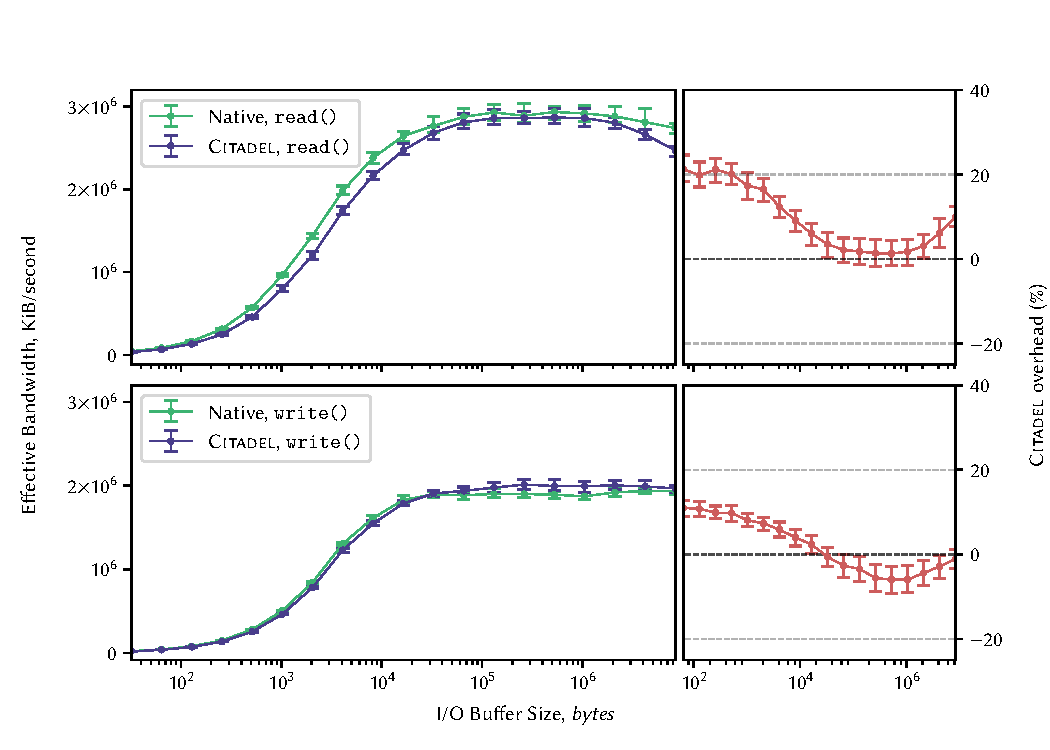
\includegraphics[width=\linewidth]{figures/graphs/io.pdf}
    \vspace{-5mm}
    \caption[Effective \texttt{read()/write()} bandwidths for both the native Linux kernel and \textsc{Citadel}.]{Effective \texttt{read()/write()} bandwidths for both the native Linux kernel and \textsc{Citadel}. The percentage overhead is also presented.}
    \label{fig:io-graph}
\end{figure}


\begin{figure}[]
    \centering
    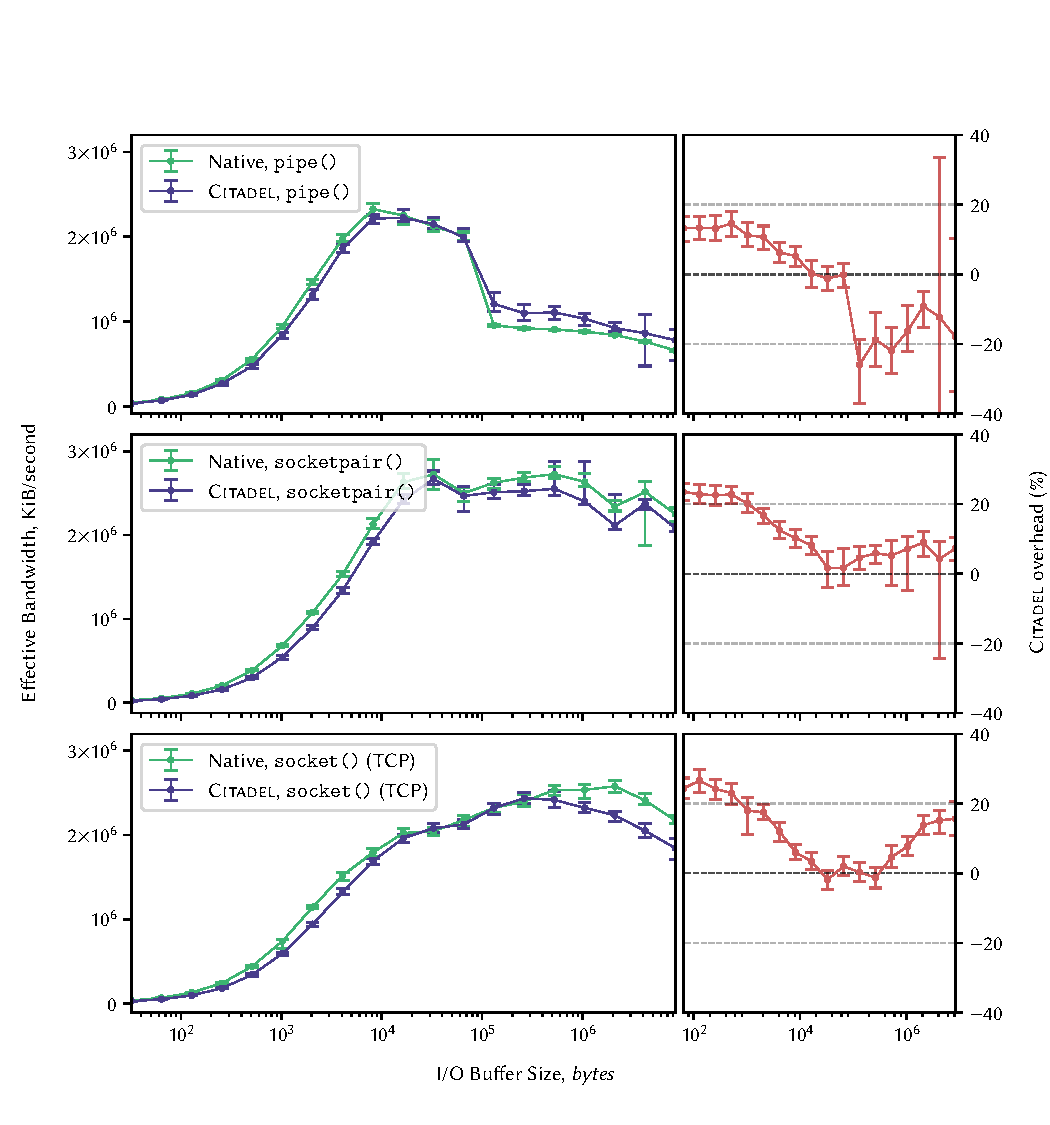
\includegraphics[width=\linewidth]{figures/graphs/ipc-2thread.pdf}
    \vspace{-5mm}
    \caption{Effective bandwidths for various types of IPC between \textit{2 threads}.}
    \label{fig:ipc-2thread-graph}
\end{figure}


\begin{figure}[]
    \centering
    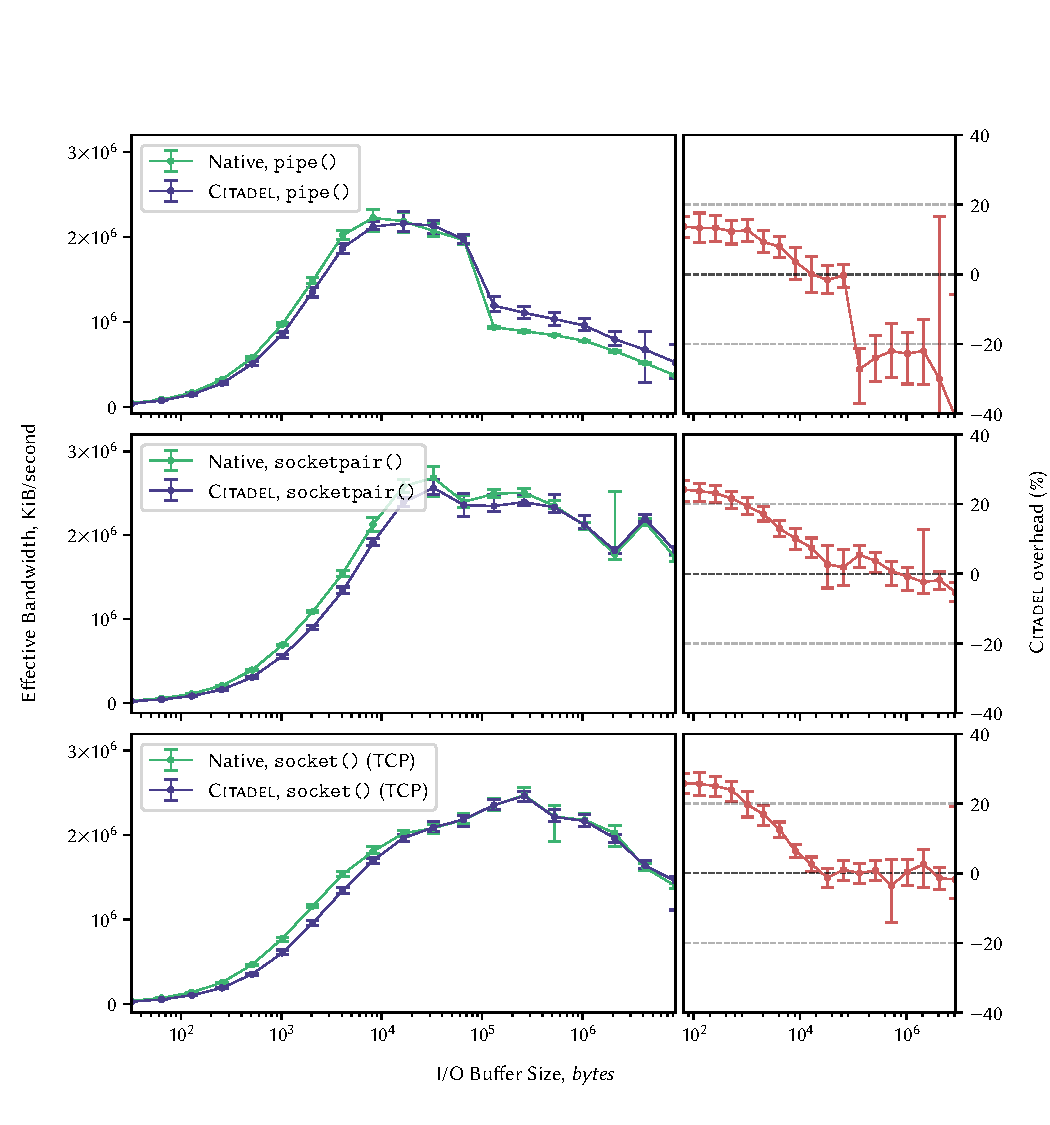
\includegraphics[width=\linewidth]{figures/graphs/ipc-2proc.pdf}
    \vspace{-5mm}
    \caption{Effective bandwidths for various types of IPC between \textit{2 processes}.}
    \label{fig:ipc-2proc-graph}
\end{figure}